\documentclass[openany]{article}
\usepackage[a4paper,margin=1in,bottom=1.5in]{geometry} % define margins. Bottom margin is used to lift a little bit the page number.
\usepackage[english]{babel} % document language is english
\usepackage{tikz} % for drawing (currently not used).
\usepackage{graphicx} % for including images
\usepackage[export]{adjustbox}
\usepackage{fancyhdr} % used for creating headers and footers. only used in title page in this document.
\usepackage{tabularx} % creation of more complex tables
\usepackage{array} % allow elements of tabular environment to have vertical alignment, e.g., center alignment.
\usepackage{nameref} % make it possible to reference by name
\usepackage{hyperref} % allow hiperlinks (links to other document parts and extern links)
\usepackage{etoc} % used for generation of section local table of contents
\usepackage{placeins}

% Define graphics path
\graphicspath{{figs/}}

% Configure the cross reference hyper links color
\hypersetup{
    colorlinks=true,
    linkcolor=blue,
}

\newcolumntype{C}{>{\centering\arraybackslash}X} % new column type for tabularx
						 % centered (\centering), adjust width in order to fill table width (X type)

% Configure header in 'titlepage'
\pagestyle{fancy}
\lhead{
\includegraphics[width=4.5cm]{logo_cnpem}}
\rhead{
\includegraphics[width=4cm]{logo_lnls}}
\renewcommand{\headrulewidth}{0pt}
\setlength{\headheight}{52pt}
% Clean footer
\fancyfoot{}

% increase table height factor a little bit (taller cells)
\renewcommand{\arraystretch}{1.5}

%==== Begin DOCUMENT ====
\begin{document}

%--- Begin title page ---
\begin{titlepage}

% Add header to this page
\thispagestyle{fancy}

% Center elements
\begin{center}

% title of title page
\topskip0pt % perfectly centered
\vspace*{\fill}
\textbf{\Huge STD-EVO Hardware Manual}\\[20pt]
\textbf{\Huge Version 1.0}\\[20pt]
\textbf{\Huge February/2017}
\vspace*{\fill}

% footer of title page
\vfill
\textbf{Beam Diagnostics Group (DIG)}\\[5pt]
\textbf{Brazilian Synchrotron Light Laboratory (LNLS)}\\[5pt]
\textbf{Brazilian Center for Research in Energy and Materials (CNPEM)}
\end{center}

\end{titlepage}
%--- End of title page ---

\newpage
\pagestyle{plain} % restore default page style

%--- About this manual ---
\paragraph{}{\Large\bfseries About this manual}

\paragraph{} This manual is intended for people who need information about the STD-EVO hardware. Information about the Timing System structure and operation, firmware, or software can be found in the corresponding manuals.

%--- Table of contents ---
\tableofcontents

\newpage
%--- Section: Important Parameters ---
\section{Important Parameters}

\begin{itemize}
\item 9 SFP connectors in the front panel (OUT0 - OUT7 and UPLINK).
\item External RF clock can be divided by 1 - 16 in STD-EVO.
\item External RF clock frequency range is 60 - 540MHz.
\item Event clock frequency range is 60 - 135MHz.
\end{itemize}

%--- Section: Hardware Specification ---
\section{Hardware Specification}

\par STD-EVO is a 19 inches 1U module. \\ 110/220V 50/60Hz AC power supply. \\
{\bfseries\color{red}NOTE: When configured as EVG, RF input should be always available before power on.}

% EVO figure
\begin{figure}[!h]
\caption{STD-EVO}
\label{fig:std-evo}
\centering
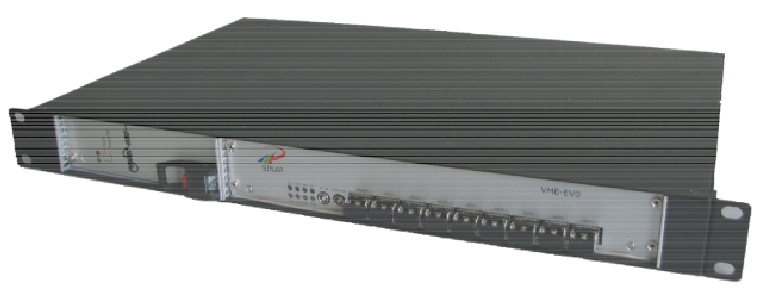
\includegraphics[width=0.7\textwidth]{std-evo-image}
\end{figure}

	% Specification table - Connectors - front panel
	\begin{table}[!h]
	  \centering
	  \caption{STD-EVO front panel connectors}
	  \label{tab:front-panel-connectors}
	  \begin{tabular}{| m{3.5cm} m{4.0cm} m{7.0cm} |}
	    \hline
	    \bfseries Connector & \bfseries Type & \bfseries Description / Specification \\ \hline

	    RF IN & LEMO EPL.00.250.NTN & \begin{tabular}{@{}m{6cm}@{}}
					  RF input \\
	    				  0 - 10dBm, 60MHz - 540MHz \\
				      	  50ohm impedance
					  \end{tabular} \\ \hline

	    AC IN / INH & LEMO EPL.00.250.NTN & \begin{tabular}{@{}m{6cm}@{}}
						AC line input (as EVG) \\
						Interlock input (as EVR) \\
						TTL level \\
	    					50ohm impedance
						\end{tabular} \\ \hline
	    UPLINK & LC Duplex & Fiber for uplink \\ \hline
	    OUT0 - OUT7 & LC Duplex & Fibers for downlink \\ \hline
	  \end{tabular}
	\end{table}

	% Specification table - LEDs - front panel
	\begin{table}[!h]
	  \centering
	  \caption{STD-EVO front panel LEDs}
	  \label{tab:front-panel-leds}
	  \begin{tabular}{| m{3.5cm} m{4.0cm} m{7.0cm} |}
	    \hline
	    \bfseries LED & \bfseries Type & \bfseries Description / Specification \\ \hline
	    EVG & Green LED & STD-EVO configured as EVG \\ \hline
	    EVR & Green LED & STD-EVO configured as EVR \\ \hline
	    FOUT & Green LED & STD-EVO configured as FOUT \\ \hline
	    FPGA & Green LED & FPGA downloaded \\ \hline
	    INH & Red LED & \begin{tabular}{@{}m{6cm}@{}}
			    Interlock input activated (as EVR) \\
			    RF input error (as EVG)
			    \end{tabular} \\ \hline
	    ENA & Green LED & STD-EVO enabled \\ \hline
	    EVT & Yellow LED & \begin{tabular}{@{}m{6cm}@{}}
			       (Blink) Event code transmitted (as EVG) \\
	    		       (Blink) Event code received (as EVR or FOUT)
			       \end{tabular} \\ \hline
	    LINK & Green LED & Uplink established \\ \hline
	  \end{tabular}
	\end{table}

	% Specification table - Connectors - rear panel
	\begin{table}[!h]
	  \centering
	  \caption{STD-EVO rear panel connectors}
	  \label{tab:rear-panel-connectors}
	  \begin{tabular}{| m{3.5cm} m{4.0cm} m{7.0cm} |}
	    \hline
	    \bfseries Connector & \bfseries Type & \bfseries Description / Specification \\ \hline
	    ETHERNET & RJ45 & 10/100Mbit Ethernet port \\ \hline
	    RST & Button & Reset Ethernet \\ \hline
	    OTP0 & HFBR-4531/4532 & OTP0 output (Agilent HFBR-1528) \\ \hline
	    OTP1 & HFBR-4531/4532 & OTP1 output (Agilent HFBR-1528) \\ \hline
	    OTP2 & HFBR-4531/4532 & OTP2 output (Agilent HFBR-1528) \\ \hline
	    OTP3 & HFBR-4531/4532 & OTP3 output (Agilent HFBR-1528) \\ \hline
	    OTP4 & HFBR-4531/4532 & OTP4 output (Agilent HFBR-1528) \\ \hline
	    OTP5 & HFBR-4531/4532 & OTP5 output (Agilent HFBR-1528) \\ \hline
	    OTP6 & HFBR-4531/4532 & OTP6 output (Agilent HFBR-1528) \\ \hline
	    OTP7 & HFBR-4531/4532 & OTP7 output (Agilent HFBR-1528) \\ \hline
	    OTP8 & HFBR-4531/4532 & OTP8 output (Agilent HFBR-1528) \\ \hline
	    OTP9 & HFBR-4531/4532 & OTP9 output (Agilent HFBR-1528) \\ \hline
	    OTP10 & HFBR-4531/4532 & OTP10 output (Agilent HFBR-1528) \\ \hline
	    OTP11 & HFBR-4531/4532 & OTP11 output (Agilent HFBR-1528) \\ \hline
	  \end{tabular}
	\end{table}

	% Specification table - LEDs - rear panel
	\begin{table}[!h]
	  \centering
	  \caption{STD-EVO rear panel LEDs}
	  \label{tab:rear-panel-leds}
	  \begin{tabular}{| m{3.5cm} m{4.0cm} m{7.0cm} |}
	    \hline
	    \bfseries LED & \bfseries Type & \bfseries Description / Specification \\ \hline
	    PWR & Green LED & Power on \\ \hline
	  \end{tabular}
	\end{table}

\FloatBarrier
%--- Section: STD-EVO Hardware ---
\section{STD-EVO Hardware}\label{sec:evo-hardware}

\par The STD-EVO module can be configured to perform one of three different roles in the timing system. It can be configured as \emph{Event Generator} (EVG), \emph{Event Receiver} (EVR), or \emph{Fanout} (FOUT). The following sections describe each of the configurations in detail.

%--- Section table of contents ---
\etoclocalframed[1]{}

	\subsection{\hyperref[sec:evo-hardware]{STD-EVO}/EVG}

	\paragraph{} When configured as EVG, the STD-EVO is an \emph{Event Generator}. In this configuraton, it acts as the Timing System master, being able to provide events and clocks to the Timing System. The STD-EVO module has three inputs: \emph{RF IN}, \emph{ACIN INH}, and \emph{UPLINK}. The signal associated with each input for the EVG configuration is described below.
	\paragraph{} The \emph{RF IN} input receives the RF signal, allowing the \emph{Event Generator} to be synchronized with the RF frequency. The \emph{RF IN} signal also defines the \emph{event clock} frequency, which is the RF frequency divided by the \emph{RF divider}, which is user-defined. The \emph{event clock} defines the parallel clock for distributing the Timing System data frames, i.e., the frequency with which data frames are broadcast to the Timing System. Each data frame is composed of two bytes (see figure \ref{fig:data-frame-evg}). One byte contains an event code, which is used by the \emph{Event Receivers} (EVR/EVE) for generating triggers. The other byte contains clock information, and will be referred to as \emph{Distributed Bus} (\emph{DBUS}). Each bit in the \emph{Distributed Bus} contains clock information about one of the EVG's channels. Therefore, the EVG (and consequently the Timing System) is able to transmit 8 channels' clocks and a trigger simultaneously.

	\begin{figure}[!h]
	\begin{tabular}{|cccccccc|c|c|c|c|c|c|c|c|}
	\hline
	\multicolumn{8}{|c|}{\emph{Event code}} & \multicolumn{8}{c|}{\emph{DBus}} \\ \hline
	\multicolumn{8}{|c|}{8 bits} & 7 & 6 & 5 & 4 & 3 & 2 & 1 & 0 \\ \hline
	\end{tabular}
	\centering
	\caption{Timing System Data Frame}
	\label{fig:data-frame-evg}
	\end{figure}
\FloatBarrier

	\paragraph{} The \emph{ACIN} input (ACIN INH) receives the mains signal when the module operates as EVG. In this case, the \emph{ACIN} signal will be referred to as \emph{AC Line}. The \emph{AC Line} is used for sychronizing the event distribution with the mains signal. This synchronization is accomplished by the \emph{\nameref{synchronizer}} submodule, which is described in section \ref{sec:evg-event-sequencer}.
	\paragraph{} The \emph{UPLINK} input is able to receive a data frame whose event code is immediately broadcast to the Timing System.
	\paragraph{} The STD-EVO module has 8 SFP outputs in the front panel which, in EVG mode, transmit the data frames containing the event code and the \emph{Distributed Bus}. The \emph{Event Sequencer} is the EVG submodule responsible for storing event codes and distributing them in the associated timestamps. Details of the \emph{Event Sequencer} and other EVG submodules and functions will be provided later in this section.
	\paragraph{} Another feature of the EVG is \emph{Timestamp Distribution}. The EVG is able to broadcast its timestamp to the Timing System and also to transmit a PPS signal. The UTC timestamp and PPS source are user-configurable.

		\subsubsection{Event Sequencer}\label{sec:evg-event-sequencer}

			\paragraph{} The \emph{Event Sequencer} is able to transmit event codes in the Timing System in previously determined instants of time with resolution of \emph{event clock} period. Additional and finer delays can be defined in the \emph{Event Receivers}. The event codes and corresponding timestamps are stored in a \emph{Sequence RAM} (\emph{SeqRAM}), which can store up to 16384 sets of event code and timestamp (see figure \ref{fig:event-sequencer}). In order to write a set of event code and timestamp to a given address of the \emph{SeqRAM}, the \nameref{reg:evg-seqram-setting} is used, in which \emph{SEQADDR} is the \emph{Sequence RAM} address, \emph{SEQCODE} is the event code to be written, and \emph{SEQTIME} is the associated timestamp. The \emph{SeqRAM} reading and distribution of stored event codes is started by a trigger, which can be selected from \emph{Synchronizer} output, VME writing access or the output of the \emph{Event FIFO}. The trigger is also responsible for restarting the \emph{Event Sequencer} timestamp, which is a counter incremented by the \emph{Event Sequencer} running clock, which is the \emph{event clock}. When the \emph{Event Sequencer} clock count is equal to the timestamp stored in the current position of the \emph{SeqRAM}, the corresponding event code is transmitted, and then the timestamp and event code move to the next contents in the \emph{SeqRAM}. The \emph{Event Sequencer} timestamp has length of 32 bits. When the current timestamp reaches 0xFFFFFFFF, the \emph{Event Sequencer} stops and waits for the next trigger.
			\paragraph{} Some event codes are used for commanding the \emph{Event Sequencer}. The event code 0x70 makes the \emph{Event Sequencer} stop at its current position in the \emph{SeqRAM} and wait for the next trigger to continue. The code 0x7F makes the \emph{Event Sequencer} move to the beginning of the \emph{SeqRAM} and wait for a trigger. 
			\paragraph{} There are two \emph{SeqRAMs} in the \emph{Event Sequencer}, which can be alternately used. The switching between the two \emph{SeqRAMs} happen in two cases. When a write operation is executed to the \emph{\nameref{reg:evg-seqram-switch}} (\emph{SEQSW} signal), or when the running \emph{SeqRAM} reads the event code 0x7E. In both cases, the switch will cause the \emph{Event Sequencer} to start reading the other \emph{SeqRAM} from the beggining.
			\paragraph{} The complete list of special event codes is available in the \hyperref[app:special-events]{Appendix A}.

			% Event Sequencer figure
			\begin{figure}[!h]
			\caption{Event Sequencer}
			\label{fig:event-sequencer}
			\centering
			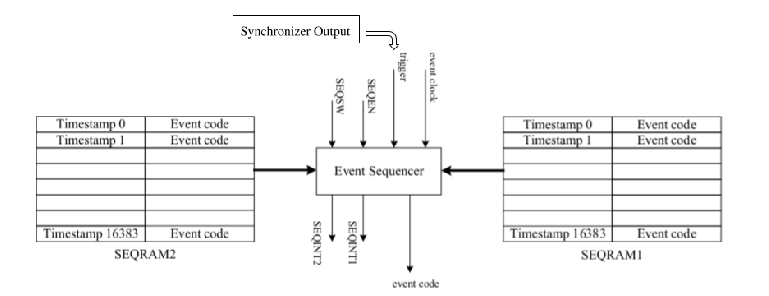
\includegraphics[width=1.0\textwidth]{event-sequencer-image}
			\end{figure}

			\paragraph{Synchronizer}\label{synchronizer} The synchronizer is responsible for providing the \emph{Event Sequencer} trigger. This trigger is the output of a D flip flop whose inputs are the \emph{AC Line} frequency and the \emph{MUX 7} divider output (see figure \ref{fig:synchronizer}). The \emph{MUX 7} divider allows for the synchronization of the \emph{AC Line} with any submultiple of the \emph{event clock}. Setting the \emph{MUX 7} divider to the \emph{Coincidence Number}, synchronizes the \emph{Event Sequencer} trigger with both the \emph{AC Line} and the {Coincidence Frequency}. The \emph{AC divider} following the D flip flop output allows the trigger frequency to be reduced to any submultiple of the mains frequency (the slowest of the synchronization frequencies).
			% Synchronizer figure
			\begin{figure}[!h]
			\caption{Synchronizer}
			\label{fig:synchronizer}
			\centering
			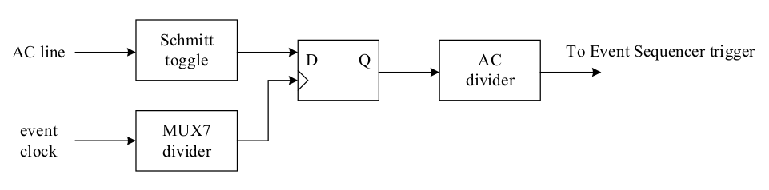
\includegraphics[width=0.7\textwidth]{synchronizer-image}
			\end{figure}

			\FloatBarrier
 
		\subsubsection{Distributed Bus}\label{sec:evg-distributed-bus}

			\paragraph{} The \emph{Distributed Bus} contains 8 clock channels, each represented by a bit in the data frame. The EVG has 8 dividers, \emph{MUX0 - MUX7}, whose outputs are mapped to the \emph{Distributed Bus} channels 0 - 7 respectively. Since the dividers input is the \emph{event clock}, each \emph{MUX} divider output, i.e., \emph{Distributed Bus} channel, is able to transmit a different submultiple of the \emph{event clock}. The configuration of the \emph{MUX} dividers and respective channels is done through the \nameref{reg:evg-mux}.

		\subsubsection{Timestamp}\label{sec:evg-timestamp}

			\paragraph{} The EVG is capable of distributing timestamps to the Timing System, allowing \emph{Event Receivers} to have accelerator-wide synchronized timestamping. The parameters and timestamp information are written/read in the \emph{\nameref{reg:evg-timestamp}}.
			\paragraph{} The Timing System 64-bit timestamp is divided in two parts. The first 32 bits hold the UTC data, containing the number of seconds passed since some epoch. This information is set by software (\emph{UTC} field) and is incremented by a user-configured PPS (Pulse Per Second) source. The EVG module is able to receive an external PPS signal (e.g., from a GPS), obtain it from the \emph{MUX 6} RF frequency divisor output, or directly from its internal oscillator. The PPS source is configured by the \emph{TIMESRC} field. There are a few circuntances when the EVG UTC timestamp is broadcast to the Timing System. The first is when a broadcast command is sent to the EVG, i.e., the value 0 is written to its \emph{UTC} field. The UTC timestamp will NOT be modified by the written 0, but the current timestamp will be broadcast. The second option for triggering a broadcast is to write a non-zero new value to the EVG's \emph{UTC} field. This will cause the timestamp to change and trigger the broadcast. The last case of timestamp broadcast happens when the EVG PPS signal source is changed. For broadcasting the timestamp, the EVG first sends the 0x74 event code, which tells the system that the UTC timestamp is going to be transmitted. The following 4 data frames contain UTC information in the event code byte. The 0x74 event resets the receivers' timestamps and guarantees that the UTC information will not be interpreted as actual event codes.
			\par Every second, the EVG sends an \emph{increment UTC} event (0x73), which may or may not be used by the \emph{Event Receivers}. If the Timing System network is uniform, the update signals reach all receivers at the same time.
			\paragraph{} The second part of the Timing System timestamp is a 32-bit subsecond counter (\emph{SUBSECOND field}). The subsecond increment signal is the \emph{event clock}, and thus, it has resolution of event clock period. Every UTC update or increment, the \emph{SUBSECOND} counter resets.

		\subsubsection{Registers}\label{sec:evg-registers}

		\begin{center}
		\renewcommand{\arraystretch}{3} % valid only in this 'center' environment
		\begin{tabular}{p{2cm} p{5cm} p{7cm}}
		\bfseries Address & \bfseries Register Name & \bfseries Description \\ \hline
		\bfseries 0 & \nameref{reg:evg-control-status} & General settings and status. Enable/disable module, \emph{Event Sequencer} status, \emph{Event Sequencer} enable/disable, and RF signal status. \\ \hline
		\bfseries 40 & \nameref{reg:evg-ac-line} & Mains signal input configuration. \emph{AC Line} enable/disable, and \emph{AC divider} setting. \\ \hline
		\bfseries 41 - 48 & \hyperref[reg:evg-mux]{MUX0 - MUX7 Register} & \emph{MUX} channels (\emph{Distributed Bus} signals) settings. MUX enable/disable, and MUX divider setting. \\ \hline
		\bfseries 49 & \nameref{reg:evg-seqram-setting} & Parameters for writing to the \emph{Sequence RAM}. \emph{SeqRAM} address, event code, and timestamp. \\ \hline
		\bfseries 50 & \nameref{reg:evg-seqram-switch} & Switch \emph{Sequence RAM}. \emph{Sequence RAM} write operations counter. \\ \hline
		\bfseries 51 & \nameref{reg:evg-timestamp} & Timestamp settings. Define PPS signal source and UTC timestamp. SUBSECOND reading.  \\ \hline
		\bfseries 62 & \nameref{reg:evg-firmware-version} & 12-byte code for current firmware version. \\ \hline
		\bfseries 63 & \nameref{reg:evg-configuration} & Main STD-EVO configuration options. Function selection (EVG, EVR, FOUT), and \emph{RF divider} setting. \\ \hline
		\end{tabular}
		\end{center}

		\paragraph{Control and Status Register}\label{reg:evg-control-status}{\large\bfseries [0]}
			
			% Reg C
			\paragraph{}{\large RegC}
			% bits 15-8
			\begin{center}
			\begin{tabularx}{0.9\textwidth}{C C C C C C C C}
			Bit 15 & Bit 14 & Bit 13 & Bit 12 & Bit 11 & Bit 10 & Bit 9 & Bit 8 \\
			% fields
			\hline
			\multicolumn{1}{|c}{} & & & \multicolumn{1}{|c}{RFINS} & \multicolumn{2}{|c|}{SEQS} & & \multicolumn{1}{c|}{} \\ \hline
	    		\end{tabularx}
			\end{center}

			\begin{center}
			% bits 7-0
			\begin{tabularx}{0.9\textwidth}{C C C C C C C C}
			Bit 7 & Bit 6 & Bit 5 & Bit 4 & Bit 3 & Bit 2 & Bit 1 & Bit 0 \\
			% fields
			\hline
			\multicolumn{1}{|c}{} & & & & & & \multicolumn{1}{|c|}{SEQEN} & \multicolumn{1}{c|}{EVGEN} \\ \hline
	    		\end{tabularx}
			\end{center}

			% Register fields description
			\bigskip
			\begin{tabular}{p{2.2cm} p{11.8cm}}
			EVGEN & Enable/Disable EVG. Disabling the EVG puts the \emph{Event Sequencer} in Stopped (idle) state, and disables \emph{MUX} channels. \\
			SEQEN & Enable/Disable the \emph{Event Sequencer}. Disabling the \emph{Event Sequencer} will return it to Stopped (idle) state. \\
			SEQS & \emph{Event Sequencer} status. \\
			& \begin{tabular}{l l}
			  0 & Stopped \\
			  1 & SEQRAM1 running \\
			  2 & SEQRAM2 running \\
			  \end{tabular} \\
			RFINS & RF input status. \\
			& \begin{tabular}{l l}
			  0 &  Loss or out of range \\
			  1 &  Normal \\
			  \end{tabular} \\
			\end{tabular}	

		\paragraph{AC line Register}\label{reg:evg-ac-line}{\large\bfseries [40]}

			% Reg A
			\paragraph{}{\large RegA}
			\begin{center}
			% bits 7-0
			\begin{tabularx}{0.9\textwidth}{C C C C C C C C}
			Bit 7 & Bit 6 & Bit 5 & Bit 4 & Bit 3 & Bit 2 & Bit 1 & Bit 0 \\
			% fields
			\hline
			\multicolumn{1}{|c}{} & & & & & & & \multicolumn{1}{|c|}{EN} \\ \hline
	    		\end{tabularx}
			\end{center}

			% Reg C
			\paragraph{}{\large RegC}
			\begin{center}
			% bits 31-0
			\begin{tabularx}{0.9\textwidth}{C C C C C C C C}
			Bit 31 & & & & & & & Bit 0 \\
			% fields
			\hline
			\multicolumn{8}{|c|}{DIV} \\ \hline
	    		\end{tabularx}
			\end{center}

			% Register fields description
			\bigskip
			\begin{tabular}{p{2.2cm} p{11.8cm}}
			EN & Enable/Disable AC Line. AC Line and event clock are the sources for the \emph{Event Sequencer} trigger. While the AC Line is disabled, the \emph{Event Sequencer} will not be triggered. \\
			DIV & AC Line divider. The divider to be applied for AC Line signal. Since \emph{ACIN} (input for AC Line) receives the mains signal, the AC Line frequency is equal to mains's (50/60Hz) divided by the AC divider. \\
			& \begin{tabular}{l}
			   {\color{red} Prescaler = DIV + 1.} \\
			   {\color{red} Example: For DIV = 0, AC Line input is divided by 1.} \\
			   \end{tabular} \\
			\end{tabular}

		\paragraph{MUXx Register}\label{reg:evg-mux}{\large\bfseries [41-48]}

			% Reg A
			\paragraph{}{\large RegA}
			\begin{center}
			% bits 7-0
			\begin{tabularx}{0.9\textwidth}{C C C C C C C C}
			Bit 7 & Bit 6 & Bit 5 & Bit 4 & Bit 3 & Bit 2 & Bit 1 & Bit 0 \\
			% fields
			\hline
			\multicolumn{1}{|c}{} & & & & & & & \multicolumn{1}{|c|}{EN} \\ \hline
	    		\end{tabularx}
			\end{center}

			% Reg C
			\paragraph{}{\large RegC}
			\begin{center}
			% bits 31-0
			\begin{tabularx}{0.9\textwidth}{C C C C C C C C}
			Bit 31 & & & & & & & Bit 0 \\
			% fields
			\hline
			\multicolumn{8}{|c|}{DIV} \\ \hline
	    		\end{tabularx}
			\end{center}

			% Register fields description
			\bigskip
			\begin{tabular}{p{2.2cm} p{11.8cm}}
			EN & Enable/Disable MUXx channel. Disabling the \emph{MUXx} channel causes the corresponding \emph{Distributed Bus} bit to remain in zero. \\
			DIV & MUXx divider. The divider to be applied for MUXx channel. The MUXx channel clock is equal to the \emph{event clock} divided by the MUXx divider. \\
			& \begin{tabular}{l}
			   {\color{red} Prescaler = DIV + 1.} \\
			   {\color{red} Example: For DIV = 0, MUXx input is divided by 1.} \\
			   \end{tabular} \\
			\end{tabular}

		\paragraph{SeqRAM Setting Register}\label{reg:evg-seqram-setting}{\large\bfseries [49]}

			% Reg A
			\paragraph{}{\large RegA}
			\begin{center}
			% bits 15-8
			\begin{tabularx}{0.9\textwidth}{C C C C C C C C}
			Bit 15 & Bit 14 & Bit 13 & Bit 12 & Bit 11 & Bit 10 & Bit 9 & Bit 8 \\
			% fields
			\hline
			\multicolumn{1}{|c}{} & & \multicolumn{6}{|c|}{SEQADDR} \\ \hline
	    		\end{tabularx}
			\end{center}

			\begin{center}
			% bits 7-0
			\begin{tabularx}{0.9\textwidth}{C C C C C C C C}
			Bit 7 & & & & & & & Bit 0 \\
			% fields
			\hline
			\multicolumn{8}{|c|}{SEQADDR} \\ \hline
	    		\end{tabularx}
			\end{center}

			% Reg B
			\paragraph{}{\large RegB}
			\begin{center}
			% bits 7-0
			\begin{tabularx}{0.9\textwidth}{C C C C C C C C}
			Bit 7 & & & & & & & Bit 0 \\
			% fields
			\hline
			\multicolumn{8}{|c|}{SEQCODE} \\ \hline
	    		\end{tabularx}
			\end{center}

			% Reg C
			\paragraph{}{\large RegC}
			\begin{center}
			% bits 31-0
			\begin{tabularx}{0.9\textwidth}{C C C C C C C C}
			Bit 31 & & & & & & & Bit 0 \\
			% fields
			\hline
			\multicolumn{8}{|c|}{SEQTIME} \\ \hline
	    		\end{tabularx}
			\end{center}

			% Register fields description
			\bigskip
			\begin{tabular}{p{2.2cm} p{11.8cm}}
			SEQADDR & The address of the waiting \emph{Sequence RAM} to receive the event code and timestamp values. \\
			SEQCODE & The event code to be written to the \emph{Sequence RAM} specified address. \\
			SEQTIME & The timestamp to be written to the \emph{Sequence RAM} specified address. \\
			\end{tabular}

		\paragraph{SeqRAM Switch Register}\label{reg:evg-seqram-switch}{\large\bfseries [50]}

			% Reg C
			\paragraph{}{\large RegC}
			\begin{center}
			% bits 15-8
			\begin{tabularx}{0.9\textwidth}{C C C C C C C C}
			Bit 15 & Bit 14 & Bit 13 & Bit 12 & Bit 11 & Bit 10 & Bit 9 & Bit 8 \\
			% fields
			\hline
			\multicolumn{1}{|c}{} & & \multicolumn{6}{|c|}{SEQCOUNT} \\ \hline
	    		\end{tabularx}
			\end{center}

			\begin{center}
			% bits 7-0
			\begin{tabularx}{0.9\textwidth}{C C C C C C C C}
			Bit 7 & & & & & & & Bit 0 \\
			% fields
			\hline
			\multicolumn{8}{|c|}{SEQCOUNT} \\ \hline
	    		\end{tabularx}
			\end{center}

			{\color{red}A write to this register switches the \emph{Sequence RAM}.}

			% Register fields description
			\bigskip
			\begin{tabular}{p{2.2cm} p{11.8cm}}
			SEQCOUNT & The number of elements in the waiting \emph{Sequence RAM}. This counter is incremented by write operations to the \emph{SeqRAM}, and reset by disabling the \emph{Event Sequencer} or the EVG. {\color{red}Read only.}\\
			\end{tabular}

		\paragraph{Timestamp Register}\label{reg:evg-timestamp}{\large\bfseries [51]}

			% Reg A
			\paragraph{}{\large RegA}
			\begin{center}
			% bits 31-0
			\begin{tabularx}{0.9\textwidth}{C C C C C C C C}
			Bit 31 & & & & & & & Bit 0 \\
			% fields
			\hline
			\multicolumn{8}{|c|}{UTC} \\ \hline
	    		\end{tabularx}
			\end{center}

			% Reg B
			\paragraph{}{\large RegB}
			\begin{center}
			% bits 31-0
			\begin{tabularx}{0.9\textwidth}{C C C C C C C C}
			Bit 31 & & & & & & & Bit 0 \\
			% fields
			\hline
			\multicolumn{8}{|c|}{SUBSECOND} \\ \hline
	    		\end{tabularx}
			\end{center}

			% Reg C
			\paragraph{}{\large RegC}
			\begin{center}
			% bits 7-0
			\begin{tabularx}{0.9\textwidth}{C C C C C C C C}
			Bit 7 & Bit 6 & Bit 5 & Bit 4 & Bit 3 & Bit 2 & Bit 1 & Bit 0 \\
			% fields
			\hline
			\multicolumn{1}{|c}{} & & & & & & \multicolumn{2}{|c|}{TIMESRC} \\ \hline
	    		\end{tabularx}
			\end{center}

			% Register fields description
			\bigskip
			\begin{tabular}{p{2.2cm} p{11.8cm}}
			UTC & The timestamp UTC field, which is a 32-bit counter to store the number of seconds passed since some epoch. The counter is incremented by the source defined in TIMESRC. A write to UTC will change the current UTC value and cause the EVG to broadcast the new timestamp. Writing zero to UTC causes the EVG to broadcast the UTC timestamp without changing its current value. The UTC broadcast, in addition to updating \emph{Event Receivers}'s UTCs, is reponsible for resetting all \emph{Event Receivers}'s SUBSECOND. \\
			SUBSECOND & The timestamp subsecond field, which is a 32-bit counter to store the subsecond portion of the Timing System timestamp. SUBSECOND is incremented by the \emph{event clock}, and thus, it has \emph{event clock} period resolution. The SUBSECOND is reset by any change of the UTC value, i.e., register access or PPS signal. The timestamp subsecond portion is not broadcast to the Timing System. \\
			TIMESRC & The PPS source. The Pulse-per-second signal is responsible for incrementing the timestamp UTC, and can be obtained from the MUX6 divider output (also \emph{DBUS6}), from an external source (rear panel PPS input), or from the internal oscillator. \\
				& \begin{tabular}{l l}
				0 & Idle. \\
				1 & DBUS (MUX6). \\
				2 & External Source. \\
				3 & Internal. \\
				\end{tabular} \\
			\end{tabular}

		\paragraph{Firmware Version Register}\label{reg:evg-firmware-version}{\large\bfseries [62]}

			% Reg A
			\paragraph{}{\large RegA}
			\begin{center}
			% bits 31-0
			\begin{tabularx}{0.9\textwidth}{C C C C C C C C}
			Bit 31 & & & & & & & Bit 0 \\
			% fields
			\hline
			\multicolumn{8}{|c|}{FRMVERSION} \\ \hline
	    		\end{tabularx}
			\end{center}

			% Reg B
			\paragraph{}{\large RegB}
			\begin{center}
			% bits 31-0
			\begin{tabularx}{0.9\textwidth}{C C C C C C C C}
			Bit 31 & & & & & & & Bit 0 \\
			% fields
			\hline
			\multicolumn{8}{|c|}{FRMVERSION} \\ \hline
	    		\end{tabularx}
			\end{center}
		
			% Reg C
			\paragraph{}{\large RegC}
			\begin{center}
			% bits 31-0
			\begin{tabularx}{0.9\textwidth}{C C C C C C C C}
			Bit 31 & & & & & & & Bit 0 \\
			% fields
			\hline
			\multicolumn{8}{|c|}{FRMVERSION} \\ \hline
	    		\end{tabularx}
			\end{center}

			% Register fields description
			\bigskip
			\begin{tabular}{p{2.2cm} p{11.8cm}}
			FRMVERSION & The STD-EVO current firmware version, which is represented by the first 12 characters of the firmware commit hash. \\
			\end{tabular}

		\paragraph{Configuration Register}\label{reg:evg-configuration}{\large\bfseries [63]}

			% Reg A
			\paragraph{}{\large RegA}
			\begin{center}
			% bits 31-0
			\begin{tabularx}{0.9\textwidth}{C C C C C C C C}
			Bit 31 & & & & & & & Bit 0 \\
			% fields
			\hline
			\multicolumn{8}{|c|}{ALIVE} \\ \hline
	    		\end{tabularx}
			\end{center}

			% Reg B
			\paragraph{}{\large RegB}
			\begin{center}
			% bits 23-16
			\begin{tabularx}{0.9\textwidth}{C C C C C C C C}
			Bit 23 & Bit 22 & Bit 21 & Bit 20 & Bit 19 & Bit 18 & Bit 17 & Bit 16 \\
			% fields
			\hline
			\multicolumn{1}{|c}{} & & & & \multicolumn{4}{|c|}{RFDIV} \\ \hline
	    		\end{tabularx}
			\end{center}

			\begin{center}
			% bits 15-8
			\begin{tabularx}{0.9\textwidth}{C C C C C C C C}
			Bit 15 & & & & & & & Bit 8 \\
			% fields
			\hline
			\multicolumn{8}{|c|}{} \\ \hline
	    		\end{tabularx}
			\end{center}

			\begin{center}
			% bits 7-0
			\begin{tabularx}{0.9\textwidth}{C C C C C C C C}
			Bit 7 & & & & & & & Bit 0 \\
			% fields
			\hline
			\multicolumn{8}{|c|}{} \\ \hline
	    		\end{tabularx}
			\end{center}

			% Reg C
			\paragraph{}{\large RegC}
			\begin{center}
			% bits 7-0
			\begin{tabularx}{0.9\textwidth}{C C C C C C C C}
			Bit 7 & Bit 6 & Bit 5 & Bit 4 & Bit 3 & Bit 2 & Bit 1 & Bit 0 \\
			% fields
			\hline
			\multicolumn{1}{|c}{0} & \multicolumn{1}{|c}{0} & \multicolumn{1}{|c}{0} & \multicolumn{1}{|c}{1} & \multicolumn{1}{|c}{0} & \multicolumn{1}{|c}{0} & \multicolumn{2}{|c|}{FUNSEL} \\ \hline
	    		\end{tabularx}
			\end{center}

			% Register fields description
			\bigskip
			\begin{tabular}{p{2.2cm} p{11.8cm}}
			ALIVE & The alive counter is incremented by the internal oscillator. It starts once the STD-EVO function is configured as EVG, EVR, or FOUT. \\
			RFDIV & The RF divider. The divider to be applied to \emph{RF IN} input signal. The output of the RF divider is the \emph{event clock}, which is the parallel clock for data frame transmission in the Timing System, the \emph{Event Sequencer} clock, and the \emph{MUX} dividers input. \\
			& \begin{tabular}{l}
			   {\color{red} Prescaler = RFDIV + 1.} \\
			   {\color{red} Example: For RFDIV = 0, RF input is divided by 1.} \\
			   \end{tabular} \\
			FUNSEL & STD-EVO function selection. \\
			& \begin{tabular}{l l}
			   0 & FOUT (default) \\
			   1 & EVR \\
			   2 & EVG \\
			   \end{tabular} \\
			\end{tabular}

			\bigskip
			\setlength{\fboxsep}{8pt}
			\fbox{\parbox[c][\height][c]{0.75\textwidth}{\emph{RFDIV} MUST be set to a valid value, i.e., that keeps \emph{event clock} within bounds, whenever the RF signal is recovered after a loss (\emph{RFINS} equal \emph{0}). If \emph{RFDIV} is not reset after RF is recovered, even if the current divider value is valid, the module will remain in Error state.} }

	\subsection{\hyperref[sec:evo-hardware]{STD-EVO}/EVR}

		\paragraph{} When configured as EVR, the STD-EVO is an \emph{Event Receiver}. The role of an \emph{Event Receiver} is to convert the data frames broadcast by the \emph{Event Generator} (EVG) into trigger and clock signals that can be transmitted to devices in the accelerator. The STD-EVO module has three inputs in the front panel, two of which are used in the EVR configuration: \emph{UPLINK}, and \emph{ACIN INH}. The signal associated with each input is described below.
		\paragraph{} The \emph{UPLINK} input is connected to one of the EVG's SFP outputs (generally with fiber optic cables). This input receives data frames broadcast by the EVG containing timing information to be converted into triggers and clocks.
		\paragraph{} The \emph{INH} input (ACIN INH) is an interlock active-low input.
		\paragraph{} The Timing System data frame is composed of two parts of 8 bits each: the event code, which is converted by the EVR into a trigger, and the \emph{Distributed Bus} (\emph{DBUS}), which carries information of 8 different clocks (see figure \ref{fig:data-frame-evr}). The parallel frequency for transmission of data frames by the EVG is defined by the EVG's \emph{event clock}, which is a submultiple of the RF frequency. In addition to obtaining the event code and \emph{Distributed Bus} clocks, the \emph{Event Receiver} uses the received data frames to recover the \emph{event clock} and lock itself to the EVG's reference clock.

		\begin{figure}[!h]
		\begin{tabular}{|cccccccc|c|c|c|c|c|c|c|c|}
		\hline
		\multicolumn{8}{|c|}{\emph{Event code}} & \multicolumn{8}{c|}{\emph{DBus}} \\ \hline
		\multicolumn{8}{|c|}{8 bits} & 7 & 6 & 5 & 4 & 3 & 2 & 1 & 0 \\ \hline
		\end{tabular}
		\centering
		\caption{Timing System Data Frame}
		\label{fig:data-frame-evr}
		\end{figure}
\FloatBarrier


		\paragraph{} The EVR has 8 SFP outputs in the front panel (OUT0 - OUT7). Each OUTx can be configured to output one of the \emph{Distributed Bus} clocks, or transmit one of the configured triggers.
		\paragraph{} The EVR triggers are configured through 24 independent channels (OTP channels). Each OTP channel can be configured to generate a trigger in response to the reception of a given event. The OTP channel also has other parameters, which define the characteristics of the output trigger, i.e., delay, width, polarity, and number of pulses.
		\paragraph{} The EVR has 12 outputs in the rear panel, which are permanently mapped to the OTP0 - OTP11 outputs, respectively.
		\paragraph{} The \emph{Event Receiver} has timestamping functinality. It has a timestamp register containing the current UTC timestamp, which is incremented through special event codes, or the \emph{Distributed Bus} bit 6 (DBUS 6) clock, depending on the configuration. The timestamp register contains a subsecond counter as well. This counter is updated by the \emph{event clock} recovered from the \emph{UPLINK}. The module has also a timestamp FIFO for storing event codes and the timestamp in which they were received. The \emph{OTP channels} have a parameter which tells whether the event being monitored should be stored upon reception.
		\paragraph{} Details of the EVR submodules are provided later in this section.

		\subsubsection{Clock Recovery}\label{sec:evr-clock-recovery}

			\paragraph{} The \emph{Event Generator} broadcasts the event code and \emph{Distributed Bus} data frame every event clock period, even when there is no event scheduled, in which case a dummy event with code 0 is broadcast. The data frame is broadcast using 8b10b encoding (see figure \ref{fig:encoding-decoding}). The \emph{Event Receivers} use the data frames that arrive from the \emph{UPLINK} to recover the \emph{event clock}.

			% Encoding-decoding figure
			\begin{figure}[!h]
			\caption{Timing system encoding-decoding scheme}
			\label{fig:encoding-decoding}
			\centering
			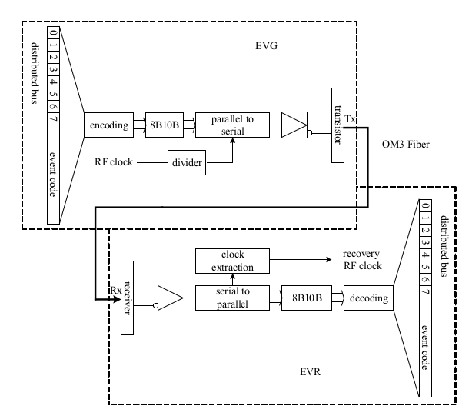
\includegraphics[width=0.7\textwidth]{encoding-decoding-image}
			\end{figure}
\FloatBarrier

		\subsubsection{Trigger Generation}\label{sec:evr-trigger-generation}

			\paragraph{} The EVR has 24 \emph{OTP} channels, each of which can be configured to generate a trigger upon the reception of a given event. The OTP channels parameters are configured in the \nameref{reg:evr-otp}.
			The \emph{EVT} parameter specifies the event code responsible for generating the trigger.
			The \emph{DELAY} parameter specifies the delay between the event reception and the output trigger in \emph{event clock} period units.
			The \emph{WIDTH} parameter specifies the width of the pulse generated in \emph{event clock} period units.
			The \emph{POL} parameter specifies the pulse polarity.
			The \emph{PULSES} parameter specifies the number of pulses to be generated in response to the event reception. When \emph{PULSES} is greater than one, the trigger generated is in fact a pulse train. The pulse train period is 2 times \emph{WIDTH} and the duty cycle is 0.5.
			\paragraph{} The EVR's \emph{Timestamp FIFO} can store the instant when some event is received. Each \emph{OTP} channel has a \emph{TIME} parameter that enables the timestamping function for the event code being monitored.

		\subsubsection{SFP Ouputs}\label{sec:evr-sfp-outputs}

			\paragraph{} The SFP outputs correspond to the OUT0 - OUT7 outputs in the EVR front panel. The OUT0 - OUT7 outputs can be configured in the \nameref{reg:evr-out}. The \emph{OUTx} signal source can be mapped to one of the \emph{OTP} channels, or any of the \emph{Distributed Bus} clocks. The source selection is defined by the \emph{SEL} parameter.
			\par The \emph{ITL} parameter enables/disables the interlock function for the corresponding \emph{OUT} channel. When the \emph{OUTx} channel has ITL \emph{enabled}, the channel is inhibited whenever the EVR's interlock input (\emph{INH}) is active (active-low signal).
			\paragraph{} The OUTx signal has an associated RF delay (\emph{RFDLY}) and fine delay (\emph{FINEDLY}). The RF delay resolution is \(\frac{1}{20}\) of \emph{event clock} period. When the value of \emph{RFDLY} is set to 31, the RF delay of the OUTx output is set by the EVG's \emph{Event Sequencer} special event codes 0x40 - 0x53, which set the delay value from 0 to 19 respectively. The RF delay special event codes can be written to the EVG's \emph{Sequence RAM}, in order to give event timestamps enough resolution to, for example, allow single bucket injection. The fine delay resolution is 5ps, and may be used for fine adjustment of the trigger timing.

		\subsubsection{POF Ouputs}\label{sec:evr-pof-outputs}

			\paragraph{} There are 12 Plastic Optical Fiber (POF) outputs in the EVR rear panel. The POF outputs are permanently mapped to the OTP0 - OTP11 channels outputs.

		\subsubsection{Timestamp}\label{sec:evr-timestamp}
		
			\paragraph{} The EVR has timestamping function, which allows it to register when events of interest are received. To this end, the module maintains a timestamp register containing the 64-bit Timing System timestamp, which comprises a 32-bit \emph{UTC} timestamp and a 32-bit \emph{SUBSECOND} timestamp. The EVG sets the EVR's timestamp (generally once), and then increments it every second. The timestamp settings and status can be accessed in the \nameref{reg:evr-timestamp}.
			\paragraph{} The 32-bit \emph{UTC} timestamp stores the number of seconds passed since some epoch. This value can only be modified by a timestamp broadcast. When the EVG broadcasts its UTC timestamp, the EVR first receives the special event code 0x74. The event 0x74 resets the \emph{SUBSECOND} counter and tells the EVR to treat the next 4 events as UTC information, instead of actual event codes. The UTC information received then replaces the current 4-byte \emph{UTC} value.
			\paragraph{} The \emph{SUBSECOND} counter is incremented by the recovered \emph{event clock}, providing \emph{event clock} period resolution to the timestamp.
			\paragraph{} The \emph{TIMESRC} field specifies the PPS source, i.e., the signal which is going to increment the EVR's UTC. When \emph{TIMESRC} is configured as \emph{EVENT}, the \emph{UTC} field is incremented by the special event 0x73, which is sent at the start of every second. When the \emph{TIMESRC} is configured as \emph{DBUS}, the \emph{UTC} field is incremented by the \emph{DBUS 6} clock. When \emph{TIMESRC} is \emph{INTERNAL}, the internal oscillator provides the increment signal. Once a PPS is received, the \emph{SUBSECOND} counter is reset and the \emph{UTC} timestamp is incremented.
			\paragraph{} In addition to the timestamp special events already mentioned, there are also event code 0x71, which resets the \emph{SUBSECOND} timestamp, and event code 0x72, which resets the \emph{UTC} timestamp.

			\paragraph{Timestamp FIFO} The EVR has a \emph{Timestamp FIFO}, also referred to as \emph{Timestamp Log}, capable of storing 16384 sets of event code and timestamp (32-bit \emph{UTC} and 32-bit \emph{SUBSECOND}). The purpose of the \emph{Timestamp Log} is to store the instant when relevant events are received. The \nameref{reg:evr-timestamp-log} is used to read and command the \emph{Timestamp FIFO}. Each \hyperref[sec:evr-trigger-generation]{OTP channel} has a timestamping setting, defining whether the event code mapped to that channel should be stored along with its timestamp once received.
			\paragraph{} The \emph{Timestamp FIFO} operates as a circular buffer, replacing the oldest timestamp value by the newest, in the case that the FIFO is full and a new timestamp is stored.
			The \emph{EMPTY} and \emph{FULL} flags indicate when the FIFO is empty, or full respectively.
			\paragraph{} Writing to the \emph{PULL} field pulls the \emph{Timestamp Log} oldest value. Reading \emph{PULL} has no effect. The pull action updates the \emph{Timestamp Log}'s \emph{UTC}, \emph{SUBSECOND}, and \emph{EVENT} fields with the UTC, subsecond, and event code obtained from the \emph{Timestamp FIFO}. The pulled information is erased from the Log. The procedure for reading the \emph{Timestamp Log} consists of writing to \emph{PULL} and reading the Log's \emph{UTC}, \emph{SUBSECOND}, and \emph{EVENT} fields.
			\paragraph{} The \emph{LOGCOUNT} field indicates how many sets of event code and timestamp are stored in the \emph{Timestamp FIFO}.
			The \emph{RSTLOG} field resets the \emph{Timestamp FIFO}, i.e., clear all stored values. The \emph{STOPLOG} field stops the timestamping function while set. Both \emph{RSTLOG} and \emph{STOPLOG} return their current value when read.

		\subsubsection{Registers}\label{sec:evr-registers}

			\begin{center}
			\renewcommand{\arraystretch}{3} % valid only in this 'center' environment
			\begin{tabular}{p{2cm} p{5cm} p{7cm}}
			\bfseries Address & \bfseries Register Name & \bfseries Description \\ \hline
			\bfseries 0 & \nameref{reg:evr-control-status} & General settings and status. Enable/disable module, \emph{UPLINK} status, and interlock input status. \\ \hline
			\bfseries 1-16 \hspace*{\fill}25-32 & \nameref{reg:evr-otp} & OTPx settings. Specifies OTPx trigger delay, width, polarity, number of pulses, and mapped event. Also enables/disables timestamping option. \\ \hline
			\bfseries 17-24 & \nameref{reg:evr-out} & OUTx settings. Specifies OUTx output signal source, RF delay, and fine delay. Also enables/disables the interlock function for the channel being configured. \\ \hline
			\bfseries 51 & \nameref{reg:evr-timestamp} & Timestamp information and settings. Define PPS signal source, reading of \emph{UTC} and \emph{SUBSECOND} values.  \\ \hline
			\bfseries 52 & \nameref{reg:evr-timestamp-log} & Timestamp Log settings. \emph{Timestamp FIFO} reading and commanding. \\ \hline
			\bfseries 62 & \nameref{reg:evr-firmware-version} & 12-byte code for current firmware version. \\ \hline
			\bfseries 63 & \nameref{reg:evr-configuration} & Main STD-EVO configuration options. Function selection (EVG, EVR, FOUT), and \emph{Clock mode} setting. \\ \hline
			\end{tabular}
			\end{center}
	
			\paragraph{Control and Status Register}\label{reg:evr-control-status}{\large\bfseries [0]}

				% Reg C
				\paragraph{}{\large RegC}
				% bits 15-8
				\begin{center}
				\begin{tabularx}{0.9\textwidth}{C C C C C C C C}
				Bit 15 & Bit 14 & Bit 13 & Bit 12 & Bit 11 & Bit 10 & Bit 9 & Bit 8 \\
				% fields
				\hline
				\multicolumn{1}{|c}{LINK} & \multicolumn{1}{|c|}{INHS} & & & & & & \multicolumn{1}{c|}{} \\ \hline
		    		\end{tabularx}
				\end{center}

				\begin{center}
				% bits 7-0
				\begin{tabularx}{0.9\textwidth}{C C C C C C C C}
				Bit 7 & Bit 6 & Bit 5 & Bit 4 & Bit 3 & Bit 2 & Bit 1 & Bit 0 \\
				% fields
				\hline
				\multicolumn{1}{|c}{} & & & & & & & \multicolumn{1}{|c|}{EVREN} \\ \hline
		    		\end{tabularx}
				\end{center}

				% Register fields description
				\bigskip
				\begin{tabular}{p{2.2cm} p{11.8cm}}
				EVREN & Enable/Disable EVR. Disabling the EVR disables all of its outputs. \\
				& \begin{tabular}{l l}
				0 & Disable \\
				1 & Enable \\
				\end{tabular} \\
				INHS & Interlock input status. The interlock input status only affects the OUTx outpus whose interlock function is enabled. \\
				& \begin{tabular}{l l}
				  0 & Disserted \\
				  1 & Asserted \\
				  \end{tabular} \\
				LINK & \emph{UPLINK} status. \\
				& \begin{tabular}{l l}
				  0 & Unlink \\
				  1 & Link \\
				  \end{tabular} \\
				\end{tabular}

			\paragraph{OTPx Register}\label{reg:evr-otp}{\large\bfseries [1-16] [25-32]}

				\paragraph{}{\color{red} OTP0 - OTP15: Address 1 - 16}
				\paragraph{}{\color{red} OTP16 - OTP23: Address 25 - 32}

				% Reg A
				\paragraph{}{\large RegA}
				% bits 31-24
				\begin{center}
				\begin{tabularx}{0.9\textwidth}{C C C C C C C C}
				Bit 31 & Bit 30 & Bit 29 & Bit 28 & Bit 27 & Bit 26 & Bit 25 & Bit 24 \\
				% fields
				\hline
				\multicolumn{1}{|c}{EN} & \multicolumn{1}{|c}{POL} & \multicolumn{1}{|c|}{TIME} & & & & & \multicolumn{1}{c|}{} \\ \hline
		    		\end{tabularx}
				\end{center}
				
				\begin{center}
				% bits 23-16
				\begin{tabularx}{0.9\textwidth}{C C C C C C C C}
				Bit 23 & & & & & & & Bit 16 \\
				% fields
				\hline
				\multicolumn{8}{|c|}{PULSES} \\ \hline
		    		\end{tabularx}
				\end{center}

				\begin{center}
				% bits 15-8
				\begin{tabularx}{0.9\textwidth}{C C C C C C C C}
				Bit 15 & & & & & & & Bit 8 \\
				% fields
				\hline
				\multicolumn{8}{|c|}{PULSES} \\ \hline
		    		\end{tabularx}
				\end{center}

				\begin{center}
				% bits 7-0
				\begin{tabularx}{0.9\textwidth}{C C C C C C C C}
				Bit 7 & & & & & & & Bit 0 \\
				% fields
				\hline
				\multicolumn{8}{|c|}{EVT} \\ \hline
		    		\end{tabularx}
				\end{center}

				% Reg B
				\paragraph{}{\large RegB}
				\begin{center}
				% bits 31-0
				\begin{tabularx}{0.9\textwidth}{C C C C C C C C}
				Bit 31 & & & & & & & Bit 0 \\
				% fields
				\hline
				\multicolumn{8}{|c|}{DELAY} \\ \hline
		    		\end{tabularx}
				\end{center}

				% Reg C
				\paragraph{}{\large RegC}
				\begin{center}
				% bits 31-0
				\begin{tabularx}{0.9\textwidth}{C C C C C C C C}
				Bit 31 & & & & & & & Bit 0 \\
				% fields
				\hline
				\multicolumn{8}{|c|}{WIDTH} \\ \hline
		    		\end{tabularx}
				\end{center}

				% Register fields description
				\bigskip
				\begin{tabular}{p{2.2cm} p{11.8cm}}
				EN & Enable/Disable OTPx. Disabling the OTPx channel does not disable its timestamping function. \\
				& \begin{tabular}{l l}
				0 & Disable \\
				1 & Enable \\
				\end{tabular} \\
				POL & OTPx polarity. Specify the polarity of the OTPx output trigger. \\
				& \begin{tabular}{l l}
				0 & Normal \\
				1 & Inverted \\
				\end{tabular} \\
				TIME & Enable/Disable OTPx timestamping. When enabled, once the mapped event is received, the corresponding code and timestamp are stored in the \emph{Timestamp FIFO}. \\
				& \begin{tabular}{l l}
				0 & Timestamping \\
				1 & Not timestamping \\
				\end{tabular} \\
				PULSES & OTPx number of pulses. Specify the number of pulses to be generated. When the number of pulses is greater than 1, the output is a pulse train with duty cycle 0.5. \\
				EVT & OTPx mapped event. Specify the event to generate the trigger. \\
				DELAY & OTPx delay. Specify the delay between the reception of the mapped event and the trigger output. \\
				WIDTH & OTPx width. Specify the width of the trigger/pulse train pulse(s). \\
				\end{tabular}

			\paragraph{OUTx Register}\label{reg:evr-out}{\large\bfseries [17-24]}

				% Reg A
				\paragraph{}{\large RegA}
				% bits 31-24
				\begin{center}
				\begin{tabularx}{0.9\textwidth}{C C C C C C C C}
				Bit 31 & Bit 30 & Bit 29 & Bit 28 & Bit 27 & Bit 26 & Bit 25 & Bit 24 \\
				% fields
				\hline
				\multicolumn{1}{|c|}{ITL} & & & & & & & \multicolumn{1}{c|}{} \\ \hline
		    		\end{tabularx}
				\end{center}
				
				\begin{center}
				% bits 23-16
				\begin{tabularx}{0.9\textwidth}{C C C C C C C C}
				Bit 23 & & & & & & & Bit 16 \\
				% fields
				\hline
				\multicolumn{8}{|c|}{} \\ \hline
		    		\end{tabularx}
				\end{center}

				\begin{center}
				% bits 15-8
				\begin{tabularx}{0.9\textwidth}{C C C C C C C C}
				Bit 15 & & & & & & & Bit 8 \\
				% fields
				\hline
				\multicolumn{8}{|c|}{} \\ \hline
		    		\end{tabularx}
				\end{center}

				\begin{center}
				% bits 7-0
				\begin{tabularx}{0.9\textwidth}{C C C C C C C C}
				Bit 7 & Bit 6 & Bit 5 & Bit 4 & Bit 3 & Bit 2 & Bit 1 & Bit 0 \\
				% fields
				\hline
				\multicolumn{1}{|c}{} & \multicolumn{7}{|c|}{SEL} \\ \hline
		    		\end{tabularx}
				\end{center}

				% Reg B
				\paragraph{}{\large RegB}	
				\begin{center}
				% bits 15-8
				\begin{tabularx}{0.9\textwidth}{C C C C C C C C}
				Bit 15 & Bit 14 & Bit 13 & Bit 12 & Bit 11 & Bit 10 & Bit 9 & Bit 8 \\
				% fields
				\hline
				\multicolumn{1}{|c}{} & & & & & & \multicolumn{2}{|c|}{FINEDLY} \\ \hline
		    		\end{tabularx}
				\end{center}

				\begin{center}
				% bits 7-0
				\begin{tabularx}{0.9\textwidth}{C C C C C C C C}
				Bit 7 & & & & & & & Bit 0 \\
				% fields
				\hline
				\multicolumn{8}{|c|}{FINEDLY} \\ \hline
		    		\end{tabularx}
				\end{center}

				% Reg C
				\paragraph{}{\large RegC}
				\begin{center}
				% bits 7-0
				\begin{tabularx}{0.9\textwidth}{C C C C C C C C}
				Bit 7 & Bit 6 & Bit 5 & Bit 4 & Bit 3 & Bit 2 & Bit 1 & Bit 0 \\
				% fields
				\hline
				\multicolumn{1}{|c}{} & & & \multicolumn{5}{|c|}{RFDLY} \\ \hline
		    		\end{tabularx}
				\end{center}

				% Register fields description
				\bigskip
				\begin{tabular}{p{2.2cm} p{11.8cm}}
				ITL & Enable/Disable OUTx interlock function. When the interlock function is enabled, the OUTx will be inhibited while the EVR interlock input (\emph{INH}) is active. \\
				& \begin{tabular}{l l}
				  0 & Disable \\
				  1 & Enable \\
				  \end{tabular} \\
				SEL & OUTx source selection. Specifies the source of the OUTx signal from one of the \emph{OTP} channels or \emph{Distributed Bus} clocks. \\
				  & \begin{tabular}{l l}
				  0x10 - 0x1F & OTP0 - OTP15 \\
				  0x20 - 0x27 & Dbus0 - Dbus7 \\
				  0x30 - 0x37 & OTP16 - OTP23 \\
				  \end{tabular} \\
				FINEDLY & OUTx fine delay. The fine delay between the event code reception and the OUTx trigger. The fine delay unit is 5ps. \\
				RFDLY & OUTx RF delay. The RF delay between the event code reception and the OUTx trigger. The RF delay unit is \(\frac{1}{20}\) of \emph{event clock} period. When \emph{RFDLY} is set to 31, the delay is defined by \emph{Event Sequencer} event codes 0x40 - 0x53, which set the RF delay to 0 - 19, respectively. \\
				\end{tabular}

			\paragraph{Timestamp Register}\label{reg:evr-timestamp}{\large\bfseries [51]}

				% Reg A
				\paragraph{}{\large RegA}
				\begin{center}
				% bits 31-0
				\begin{tabularx}{0.9\textwidth}{C C C C C C C C}
				Bit 31 & & & & & & & Bit 0 \\
				% fields
				\hline
				\multicolumn{8}{|c|}{UTC} \\ \hline
		    		\end{tabularx}
				\end{center}

				% Reg B
				\paragraph{}{\large RegB}
				\begin{center}
				% bits 31-0
				\begin{tabularx}{0.9\textwidth}{C C C C C C C C}
				Bit 31 & & & & & & & Bit 0 \\
				% fields
				\hline
				\multicolumn{8}{|c|}{SUBSECOND} \\ \hline
		    		\end{tabularx}
				\end{center}

				% Reg C
				\paragraph{}{\large RegC}
				\begin{center}
				% bits 7-0
				\begin{tabularx}{0.9\textwidth}{C C C C C C C C}
				Bit 7 & Bit 6 & Bit 5 & Bit 4 & Bit 3 & Bit 2 & Bit 1 & Bit 0 \\
				% fields
				\hline
				\multicolumn{1}{|c}{} & & & & & & \multicolumn{2}{|c|}{TIMESRC} \\ \hline
		    		\end{tabularx}
				\end{center}

				% Register fields description
				\bigskip
				\begin{tabular}{p{2.2cm} p{11.8cm}}
				UTC & The timestamp UTC field, which is a 32-bit counter to store the number of seconds passed since some epoch. The counter is incremented by the source defined in \emph{TIMESRC}. The UTC can only be modified by EVG timestamp broadcasts or PPS signal. \\
				SUBSECOND & The timestamp subsecond field, which is a 32-bit counter to store the subsecond portion of the Timing System timestamp. SUBSECOND is incremented by the recovered \emph{event clock}, and thus, it has \emph{event clock} period resolution. The SUBSECOND is reset whenever a PPS signal or UTC broadcast is received. \\
				TIMESRC & The Pulse-per-second signal source, which is responsible for incrementing the timestamp UTC. The PPS signal can be obtained from the clock transmitted by the \emph{Distributed Bus} bit 6, from the special event code 0x73, which is broadcast by the EVG at the start of every second, or from the internal oscillator. \\
				& \begin{tabular}{l l}
				0 & Idle \\
				1 & DBUS (DBUS6) \\
				2 & Event \\
				3 & Internal \\
				\end{tabular} \\
			\end{tabular}

			\paragraph{Timestamp Log Register}\label{reg:evr-timestamp-log}{\large\bfseries [52]}

				% Reg A
				\paragraph{}{\large RegA}
				\begin{center}
				% bits 31-0
				\begin{tabularx}{0.9\textwidth}{C C C C C C C C}
				Bit 31 & & & & & & & Bit 0 \\
				% fields
				\hline
				\multicolumn{8}{|c|}{UTC} \\ \hline
		    		\end{tabularx}
				\end{center}

				% Reg B
				\paragraph{}{\large RegB}
				\begin{center}
				% bits 31-0
				\begin{tabularx}{0.9\textwidth}{C C C C C C C C}
				Bit 31 & & & & & & & Bit 0 \\
				% fields
				\hline
				\multicolumn{8}{|c|}{SUBSECOND} \\ \hline
		    		\end{tabularx}
				\end{center}

				% Reg C
				\paragraph{}{\large RegC}
				\begin{center}
				% bits 31-24
				\begin{tabularx}{0.9\textwidth}{C C C C C C C C}
				Bit 31 & & & & & & & Bit 24 \\
				% fields
				\hline
				\multicolumn{8}{|c|}{EVENT} \\ \hline
		    		\end{tabularx}
				\end{center}

				\begin{center}
				% bits 23-16
				\begin{tabularx}{0.9\textwidth}{C C C C C C C C}
				Bit 23 & & & & & & & Bit 16 \\
				% fields
				\hline
				\multicolumn{8}{|c|}{LOGCOUNT} \\ \hline
		    		\end{tabularx}
				\end{center}

				\begin{center}
				% bits 15-8
				\begin{tabularx}{0.9\textwidth}{C C C C C C C C}
				Bit 15 & & & & & & & Bit 8 \\
				% fields
				\hline
				\multicolumn{8}{|c|}{LOGCOUNT} \\ \hline
		    		\end{tabularx}
				\end{center}

				\begin{center}
				% bits 7-0
				\begin{tabularx}{0.9\textwidth}{C C C C C C C C}
				Bit 7 & Bit 6 & Bit 5 & Bit 4 & Bit 3 & Bit 2 & Bit 1 & Bit 0 \\
				% fields
				\hline
				\multicolumn{1}{|c}{STOPLOG} & \multicolumn{1}{|c}{RSTLOG} & \multicolumn{1}{|c|}{PULL} & & & & \multicolumn{1}{|c}{FULL} & \multicolumn{1}{|c|}{EMPTY} \\ \hline
		    		\end{tabularx}
				\end{center}

				% Register fields description
				\bigskip
				\begin{tabular}{p{2.2cm} p{11.8cm}}
				UTC & Last UTC timestamp pulled from the \emph{Timestamp FIFO}. \\
				SUBSECOND & Last subsecond timestamp pulled from the \emph{Timestamp FIFO}. \\
				EVENT & Last event code pulled from the \emph{Timestamp FIFO}. \\
				LOGCOUNT & Number of sets of event code and timestamp in the \emph{Timestamp FIFO}. \\
				STOPLOG & Stop log function. When enabled, the timestamping function is stopped. \\
				& \begin{tabular}{l l}
				0 & Disable \\
				1 & Enable \\
				\end{tabular} \\
				RSTLOG & Reset log function. When enabled, the \emph{Timestamp FIFO} is cleared. \\
				& \begin{tabular}{l l}
				0 & Disable \\
				1 & Enable \\
				\end{tabular} \\
				PULL & Pull timestamp from \emph{Timestamp FIFO}. Writing to \emph{PULL} moves the oldest set of event code and timestamp from the \emph{Timestamp FIFO} to the \emph{UTC}, \emph{SUBSECOND}, and \emph{EVENT} fields of the \emph{Timestamp Log Register}, where it is available for reading. \\
				FULL & \emph{Timestamp FIFO} full flag. The full flag is set while LOGCOUNT is equal to 16384. While \emph{RSTLOG} is set, both \emph{FULL} and \emph{EMPTY} flags stay in 1. \\
				& \begin{tabular}{l l}
				0 & FIFO is not full \\
				1 & FIFO is full \\
				\end{tabular} \\
				EMPTY & \emph{Timestamp FIFO} empty. The empty flag is set while LOGCOUNT is 0. While \emph{RSTLOG} is set, both \emph{FULL} and \emph{EMPTY} flags stay in 1. \\
				& \begin{tabular}{l l}
				0 & FIFO is not empty \\
				1 & FIFO is empty \\
				\end{tabular} \\
				\end{tabular}

				\bigskip
				\setlength{\fboxsep}{8pt}
				\fbox{\parbox[c][\height][c]{0.75\textwidth}{When the \emph{UPLINK} signal is lost, \emph{STOPLOG} is automatically set to 1. In this circumstance, \emph{STOPLOG} can only be disabled after a \emph{Timestamp Log} reset (\emph{RSTLOG} set to 1).} }

			\paragraph{Firmware Version Register}\label{reg:evr-firmware-version}{\large\bfseries [62]}

				% Reg A
				\paragraph{}{\large RegA}
				\begin{center}
				% bits 31-0
				\begin{tabularx}{0.9\textwidth}{C C C C C C C C}
				Bit 31 & & & & & & & Bit 0 \\
				% fields
				\hline
				\multicolumn{8}{|c|}{FRMVERSION} \\ \hline
		    		\end{tabularx}
				\end{center}

				% Reg B
				\paragraph{}{\large RegB}
				\begin{center}
				% bits 31-0
				\begin{tabularx}{0.9\textwidth}{C C C C C C C C}
				Bit 31 & & & & & & & Bit 0 \\
				% fields
				\hline
				\multicolumn{8}{|c|}{FRMVERSION} \\ \hline
		    		\end{tabularx}
				\end{center}
		
				% Reg C
				\paragraph{}{\large RegC}
				\begin{center}
				% bits 31-0
				\begin{tabularx}{0.9\textwidth}{C C C C C C C C}
				Bit 31 & & & & & & & Bit 0 \\
				% fields
				\hline
				\multicolumn{8}{|c|}{FRMVERSION} \\ \hline
		    		\end{tabularx}
				\end{center}

				% Register fields description
				\bigskip
				\begin{tabular}{p{2.2cm} p{11.8cm}}
				FRMVERSION & The STD-EVO current firmware version, which is represented by the first 12 characters of the firmware commit hash. \\
				\end{tabular}

			\paragraph{Configuration Register}\label{reg:evr-configuration}{\large\bfseries [63]}

				% Reg A
				\paragraph{}{\large RegA}
				\begin{center}
				% bits 31-0
				\begin{tabularx}{0.9\textwidth}{C C C C C C C C}
				Bit 31 & & & & & & & Bit 0 \\
				% fields
				\hline
				\multicolumn{8}{|c|}{ALIVE} \\ \hline
		    		\end{tabularx}
				\end{center}

				% Reg B
				\paragraph{}{\large RegB}
				\begin{center}
				% bits 7-0
				\begin{tabularx}{0.9\textwidth}{C C C C C C C C}
				Bit 7 & Bit 6 & Bit 5 & Bit 4 & Bit 3 & Bit 2 & Bit 1 & Bit 0 \\
				% fields
				\hline
				\multicolumn{1}{|c}{} & & & \multicolumn{5}{|c|}{CLKMODE} \\ \hline
		    		\end{tabularx}
				\end{center}

				% Reg C
				\paragraph{}{\large RegC}
				\begin{center}
				% bits 7-0
				\begin{tabularx}{0.9\textwidth}{C C C C C C C C}
				Bit 7 & Bit 6 & Bit 5 & Bit 4 & Bit 3 & Bit 2 & Bit 1 & Bit 0 \\
				% fields
				\hline
				\multicolumn{1}{|c}{0} & \multicolumn{1}{|c}{0} & \multicolumn{1}{|c}{0} & \multicolumn{1}{|c}{1} & \multicolumn{1}{|c}{0} & \multicolumn{1}{|c}{0} & \multicolumn{2}{|c|}{FUNSEL} \\ \hline
		    		\end{tabularx}
				\end{center}

				% Register fields description
				\bigskip
				\begin{tabular}{p{2.2cm} p{11.8cm}}
				ALIVE & The alive counter is incremented by the internal oscillator. It starts once the STD-EVO function is configured as EVG, EVR, or FOUT. \\
				CLKMODE & Clock mode. Set according to \emph{UPLINK} event clock frequency. \\
				& \begin{tabular}{l l}
				   11 & 60MHz - 62.5MHz \\
				   12 & 63MHz - 77MHz \\
				   13 & 77.5MHz - 91.5MHz \\
				   14 & 92MHz - 106MHz \\
				   15 & 106MHz - 120.5MHz \\
				   16 & 121MHz - 135MHz \\
				   \end{tabular} \\				
				FUNSEL & STD-EVO function selection. \\
				& \begin{tabular}{l l}
				   0 & FOUT (default) \\
				   1 & EVR \\
				   2 & EVG \\
				   \end{tabular} \\
				\end{tabular}

	\subsection{\hyperref[sec:evo-hardware]{STD-EVO}/FOUT}

		\paragraph{} When configured as FOUT, the STD-EVO is a \emph{fanout}. The role of a \emph{fanout} is to broadcast the information, i.e., data frames, received in its \emph{UPLINK} to all of its SFP outputs (OUT0 - OUT7), extending the output capability of the \emph{Event Generator} (see figure \ref{fig:fout-usage}).

		% FOUT usage figure
		\begin{figure}[!h]
		\caption{FOUT extending the EVG output}
		\label{fig:fout-usage}
		\centering
		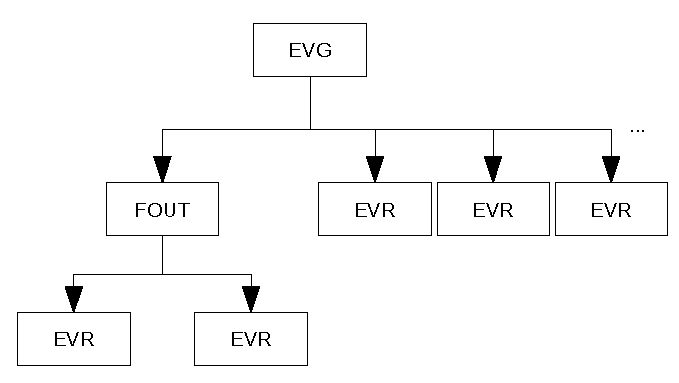
\includegraphics[width=0.7\textwidth]{fout-usage-image}
		\end{figure}

		\subsubsection{Registers}\label{sec:evr-registers}

			\begin{center}
			\renewcommand{\arraystretch}{3} % valid only in this 'center' environment
			\begin{tabular}{p{2cm} p{5cm} p{7cm}}
			\bfseries Address & \bfseries Register Name & \bfseries Description \\ \hline
			\bfseries 0 & \nameref{reg:fout-control-status} & General settings and status. Enable/disable module, \emph{UPLINK} status, and downlink status. \\ \hline
			\end{tabular}
			\end{center}

			\paragraph{Control and Status Register}\label{reg:fout-control-status}{\large\bfseries [0]}

				% Reg C
				\paragraph{}{\large RegC}
				% bits 31-24
				\begin{center}
				\begin{tabularx}{0.9\textwidth}{C C C C C C C C}
				Bit 15 & Bit 14 & Bit 13 & Bit 12 & Bit 11 & Bit 10 & Bit 9 & Bit 8 \\
				% fields
				\hline
				\multicolumn{1}{|c}{LOS0} & \multicolumn{1}{|c}{LOS1} & \multicolumn{1}{|c}{LOS2} & \multicolumn{1}{|c}{LOS3} & \multicolumn{1}{|c}{LOS4} & \multicolumn{1}{|c}{LOS5} & \multicolumn{1}{|c}{LOS6} & \multicolumn{1}{|c|}{LOS7} \\ \hline
		    		\end{tabularx}
				\end{center}

				% bits 23-16
				\begin{center}
				\begin{tabularx}{0.9\textwidth}{C C C C C C C C}
				Bit 23 & & & & & & & Bit 16 \\
				% fields
				\hline
				\multicolumn{8}{|c|}{} \\ \hline
		    		\end{tabularx}
				\end{center}

				% bits 15-8
				\begin{center}
				\begin{tabularx}{0.9\textwidth}{C C C C C C C C}
				Bit 15 & Bit 14 & Bit 13 & Bit 12 & Bit 11 & Bit 10 & Bit 9 & Bit 8 \\
				% fields
				\hline
				\multicolumn{1}{|c|}{LINK} & & & & & & & \multicolumn{1}{c|}{} \\ \hline
		    		\end{tabularx}
				\end{center}

				\begin{center}
				% bits 7-0
				\begin{tabularx}{0.9\textwidth}{C C C C C C C C}
				Bit 7 & Bit 6 & Bit 5 & Bit 4 & Bit 3 & Bit 2 & Bit 1 & Bit 0 \\
				% fields
				\hline
				\multicolumn{1}{|c}{} & & & & & & & \multicolumn{1}{|c|}{FOUTEN} \\ \hline
		    		\end{tabularx}
				\end{center}

				% Register fields description
				\bigskip
				\begin{tabular}{p{2.2cm} p{11.8cm}}
				FOUTEN & Enable/Disable FOUT. Disabling the FOUT disables all of its outputs. \\
				& \begin{tabular}{l l}
				0 & Disable \\
				1 & Enable \\
				\end{tabular} \\
				LINK & \emph{UPLINK} status. \\
				& \begin{tabular}{l l}
				  0 & Unlink \\
				  1 & Link \\
				  \end{tabular} \\
				LOS0 - LOS7 & Downlink status of OUT0 - OUT7 outputs, respectively. \\
				& \begin{tabular}{l l}
				  0 & Unlink \\
				  1 & Link \\
				  \end{tabular} \\				
				\end{tabular}

\FloatBarrier

%--- Section: Ethernet Network Interface ---
\section{Ethernet Network Interface}

	\begin{itemize}
	\item 10/100Mbit Ethernet interface.
	\item UDP protocol by default.
	\item DHCP client by default.
	\end{itemize}

%--- Section table of contents ---
\etoclocalframed[1]{}

	\subsection{Network configuration}
	
		\paragraph{} In order to modify the module's network configurations, e.g., the IP address, the Telnet program command \emph{telnet {\textless}IP address{\textgreater} 9999} can be used. Another option is to use the web browser, and type the module's IP address directly into the address bar, which will open the configuration page.

		% Telnet connection figure
		\begin{figure}[!h]
		\caption{Setup using Telnet}
		\label{fig:telnet}
		\centering
		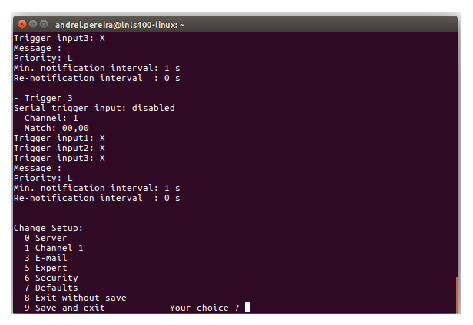
\includegraphics[width=0.7\textwidth]{telnet-image}
		\end{figure}
\FloatBarrier

	\subsection{Register Read/Write}

		\paragraph{} Both read and write operations use the same structure for the UDP data frame, which is the following:

			\bigskip
			% UDP Data Frame: byte 0-12
			\begin{tabularx}{\textwidth}{C C C C C C C C C C C C C}
			Byte 0 & Byte 1 & & & Byte 4 & Byte 5 & & & Byte 8 & Byte 9 & & & Byte 12 \\
			% fields
			\hline
			\multicolumn{1}{|c}{Command} & \multicolumn{4}{|c}{RegA} & \multicolumn{4}{|c}{RegB} & \multicolumn{4}{|c|}{RegC} \\ \hline
	    		\end{tabularx}

			\paragraph{} The \emph{RegA}, \emph{RegB}, and \emph{RegC} sections in the UDP data frame correspond to the 32-bit register sections of same name in each register. These sections carry the information to be written/read. The operation selection and register are specified by the \emph{Command} byte of the UDP data frame.

		\paragraph{Read (request)} In order to read a register, the UDP data frame \emph{Command} byte must agree with the following rule:

			\bigskip
			% Command: bits 7-0
			\begin{tabularx}{\textwidth}{C C C C C C C C}
			Bit 7 & Bit 6 & Bit 5 & Bit 4 & Bit 3 & Bit 2 & Bit 1 & Bit 0 \\
			% fields
			\hline
			\multicolumn{1}{|c}{1} & \multicolumn{1}{|c}{0} & \multicolumn{6}{|c|}{Address} \\ \hline
	    		\end{tabularx}

			\paragraph{} The first bits, from left to right, must be 1 and 0 respectively, followed by the register address.

		\paragraph{Read (response)} The response to a read request has a different \emph{Command} byte, which is represented below:

			\bigskip
			% Command: bits 7-0
			\begin{tabularx}{\textwidth}{C C C C C C C C}
			Bit 7 & Bit 6 & Bit 5 & Bit 4 & Bit 3 & Bit 2 & Bit 1 & Bit 0 \\
			% fields
			\hline
			\multicolumn{1}{|c}{1} & \multicolumn{1}{|c}{1} & \multicolumn{6}{|c|}{Address} \\ \hline
	    		\end{tabularx}		

			\paragraph{} The first bits, from left to right, must be 1 and 1 respectively, followed by the register address.

		\paragraph{Write} In order to write to a register, the UDP data frame \emph{Command} byte must agree with the following rule:

			\bigskip
			% Command: bits 7-0
			\begin{tabularx}{\textwidth}{C C C C C C C C}
			Bit 7 & Bit 6 & Bit 5 & Bit 4 & Bit 3 & Bit 2 & Bit 1 & Bit 0 \\
			% fields
			\hline
			\multicolumn{1}{|c}{0} & \multicolumn{1}{|c}{1} & \multicolumn{6}{|c|}{Address} \\ \hline
	    		\end{tabularx}
	
			\paragraph{} The first bits, from left to right, must be 0 and 1 respectively, followed by the register address.

%--- Appendices ---
\newpage
\appendix
%--- Section: Appendix A ---
\section{Special Events}\label{app:special-events}

	\begin{center}
	\begin{tabular}{|p{2cm} p{8cm}|}
	\multicolumn{1}{p{2cm}}{\bfseries Event code} & \multicolumn{1}{p{8cm}}{\bfseries Description} \\
	% events
	\hline
	\multicolumn{2}{p{10cm}}{\emph{General Purpose{\color{red}\textsuperscript{1}}}} \\ \hline
	0x00 & Idle Event \\ \hline
	\multicolumn{2}{p{10cm}}{\emph{Sequence RAM commanding}} \\ \hline
	0x70 & SEQRAM stop and wait a trigger to continue \\ \hline
	0x7E & SEQRAM switch \\ \hline
	0x7F & End of sequence, back to top \\ \hline
	\multicolumn{2}{p{10cm}}{\emph{Timestamp{\color{red}\textsuperscript{1}}}} \\ \hline
	0x71 & Reset subsecond timestamp register \\ \hline
	0x72 & Reset UTC timestamp register \\ \hline
	0x73 & Increment by 1 the UTC timestamp register and reset subsecond \\ \hline
	0x74 & Start of 32-bit UTC timestamp register update \\ \hline
	\multicolumn{2}{p{10cm}}{\emph{OUTx RF delay setting}} \\ \hline
	0x40 & delay = 0 \\ \hline
	0x41 & delay = 1 \\ \hline
	0x42 & delay = 2 \\ \hline
	0x43 & delay = 3 \\ \hline
	0x44 & delay = 4 \\ \hline
	0x45 & delay = 5 \\ \hline
	0x46 & delay = 6 \\ \hline
	0x47 & delay = 7 \\ \hline
	0x48 & delay = 8 \\ \hline
	0x49 & delay = 9 \\ \hline
	0x4A & delay = 10 \\ \hline
	0x4B & delay = 11 \\ \hline
	0x4C & delay = 12 \\ \hline
	0x4D & delay = 13 \\ \hline
	0x4E & delay = 14 \\ \hline
	0x4F & delay = 15 \\ \hline
	0x50 & delay = 16 \\ \hline
	0x51 & delay = 17 \\ \hline
	0x52 & delay = 18 \\ \hline
	0x53 & delay = 19 \\ \hline
	\end{tabular}
	\end{center}
	\par {\color{red} \textsuperscript{1}Generated by module regardless of any configuration.}

\end{document}
\grid
